% !TeX root = ../praktikum.tex
% !TeX encoding = UTF-8
% !Tex spellcheck = de_DE


Im letzten Versuchsteil wurde der Laserstrahl am anderen Ende der Glasfaser ausgekoppelt und auf einen optischen Pfad gesandt, um Abbildungen von Objekten und deren Fourierspektren, sowie die Veränderung der Abbildung bei Maniplation des Fourierspektrums zu beobachten. Hierfür wurde hinter dem Faserauskoppler der Aufbau aus Abbildung \ref{fig:4f-aufbau} realisiert.

\begin{figure}[h]
	\centering
	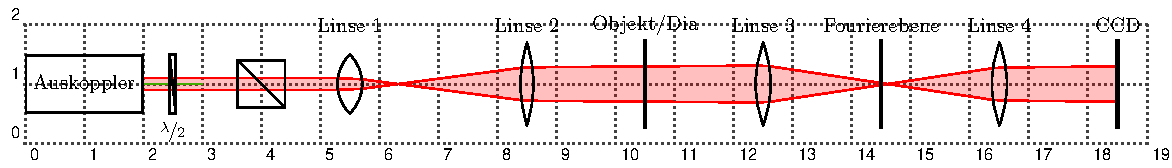
\includegraphics[width=1\linewidth]{graphs/versuchsaufbau/4f-aufbau.pdf}
	\caption[Schematische Skizze des 4f-Aufbaus]{
		Schematische Skizze des 4f-Aufbaus. Der Laserstrahl passiert nach Verlassen des Auskopplers eine $\nicefrac{\lambda}{2}$-Platte und anschließend einen Strahlteiler. Der zweite Teil des Strahls, welcher vom Strahlteiler abgelenkt wird, trifft auf eine Strahlblockierung und wird nicht weiter verwendet. Zwischen Linse 2 und 3 befindet sich die Halterung für das Objekt/Dia, in der Fourierebene wird entweder eine zweite Kamera oder ein Filter positioniert. Die CCD Kamera am Ende des Strahlengangs befindet sich in der Abbildungsebene des Aufbaus.
	}
	\label{fig:4f-aufbau}
\end{figure}

In diesem, sogenannten 4f-Aufbau, passierte der Laserstrahl nach der Reflektion am ersten Spiegel eine $\nicefrac{\lambda}{2}$-Platte und dahinter einen Strahlteiler. Mithilfe des Strahlteilers wurde eine eindeutige Polarisierung sicher gestellt, während mit dem Plättchen die Lichtmenge der durchlässigen Polarisation eingestellt werden konnte.\\

Um die abzubildenden Objekte vollständig ausleuchten zu können, wurde der Laserstrahl in diesem Aufbau mit Hilfe der ersten beiden Linsen aufgeweitet und wieder kollimiert. Im Brennpunkt der dritten Linse befand sich ein Objektträger in der Gegenstandsebene. In diesem wurden die abzubildenden Objekte angebracht. Die Fourierebene befindet sich im Brennpunkt der Linsen 3 und 4. Nach der vierten Linse wird der Strahl erneut kollimiert und trifft auf die CCD Kamera, Kamera 1. Hier wird das Objekt möglichst originalgetreu abgebildet. Um Aufnahmen der Fourierspektren zu erhalten, wurde bei Bedarf eine zweite Kamera, Kamera 2, in der Fourierebene montiert. \\ 

Verwendet wurden hierbei Linsen der Brennweiten wie folgt: Linse 1 mit $f_{1}=\unit[20]{mm}$, Linse 2 mit $f_{2}=\unit[200]{mm}$, Linse 3 und 4 mit $f_{3}=f_{4}=\unit[100]{mm}$. Direkt hinter der Auskopplung wurde zusätzlich ein Spiegel, optimiert für Wellenlängen zwischen \unit[400-700]{nm}, in den 4f-Aufbau aufgenommen, um den Verlauf des Laserstrahls im optischen Pfad besser feinjustieren zu können. Leider wurde die Strahlqualität durch diesen stark beeinträchtigt, so dass zusätzlich ein Pinhole zwischen Linse 1 und 2 notwendig war, um eine gaußähnliche Strahlmode zu erhalten.\\


\begin{figure}[h]
	\centering
	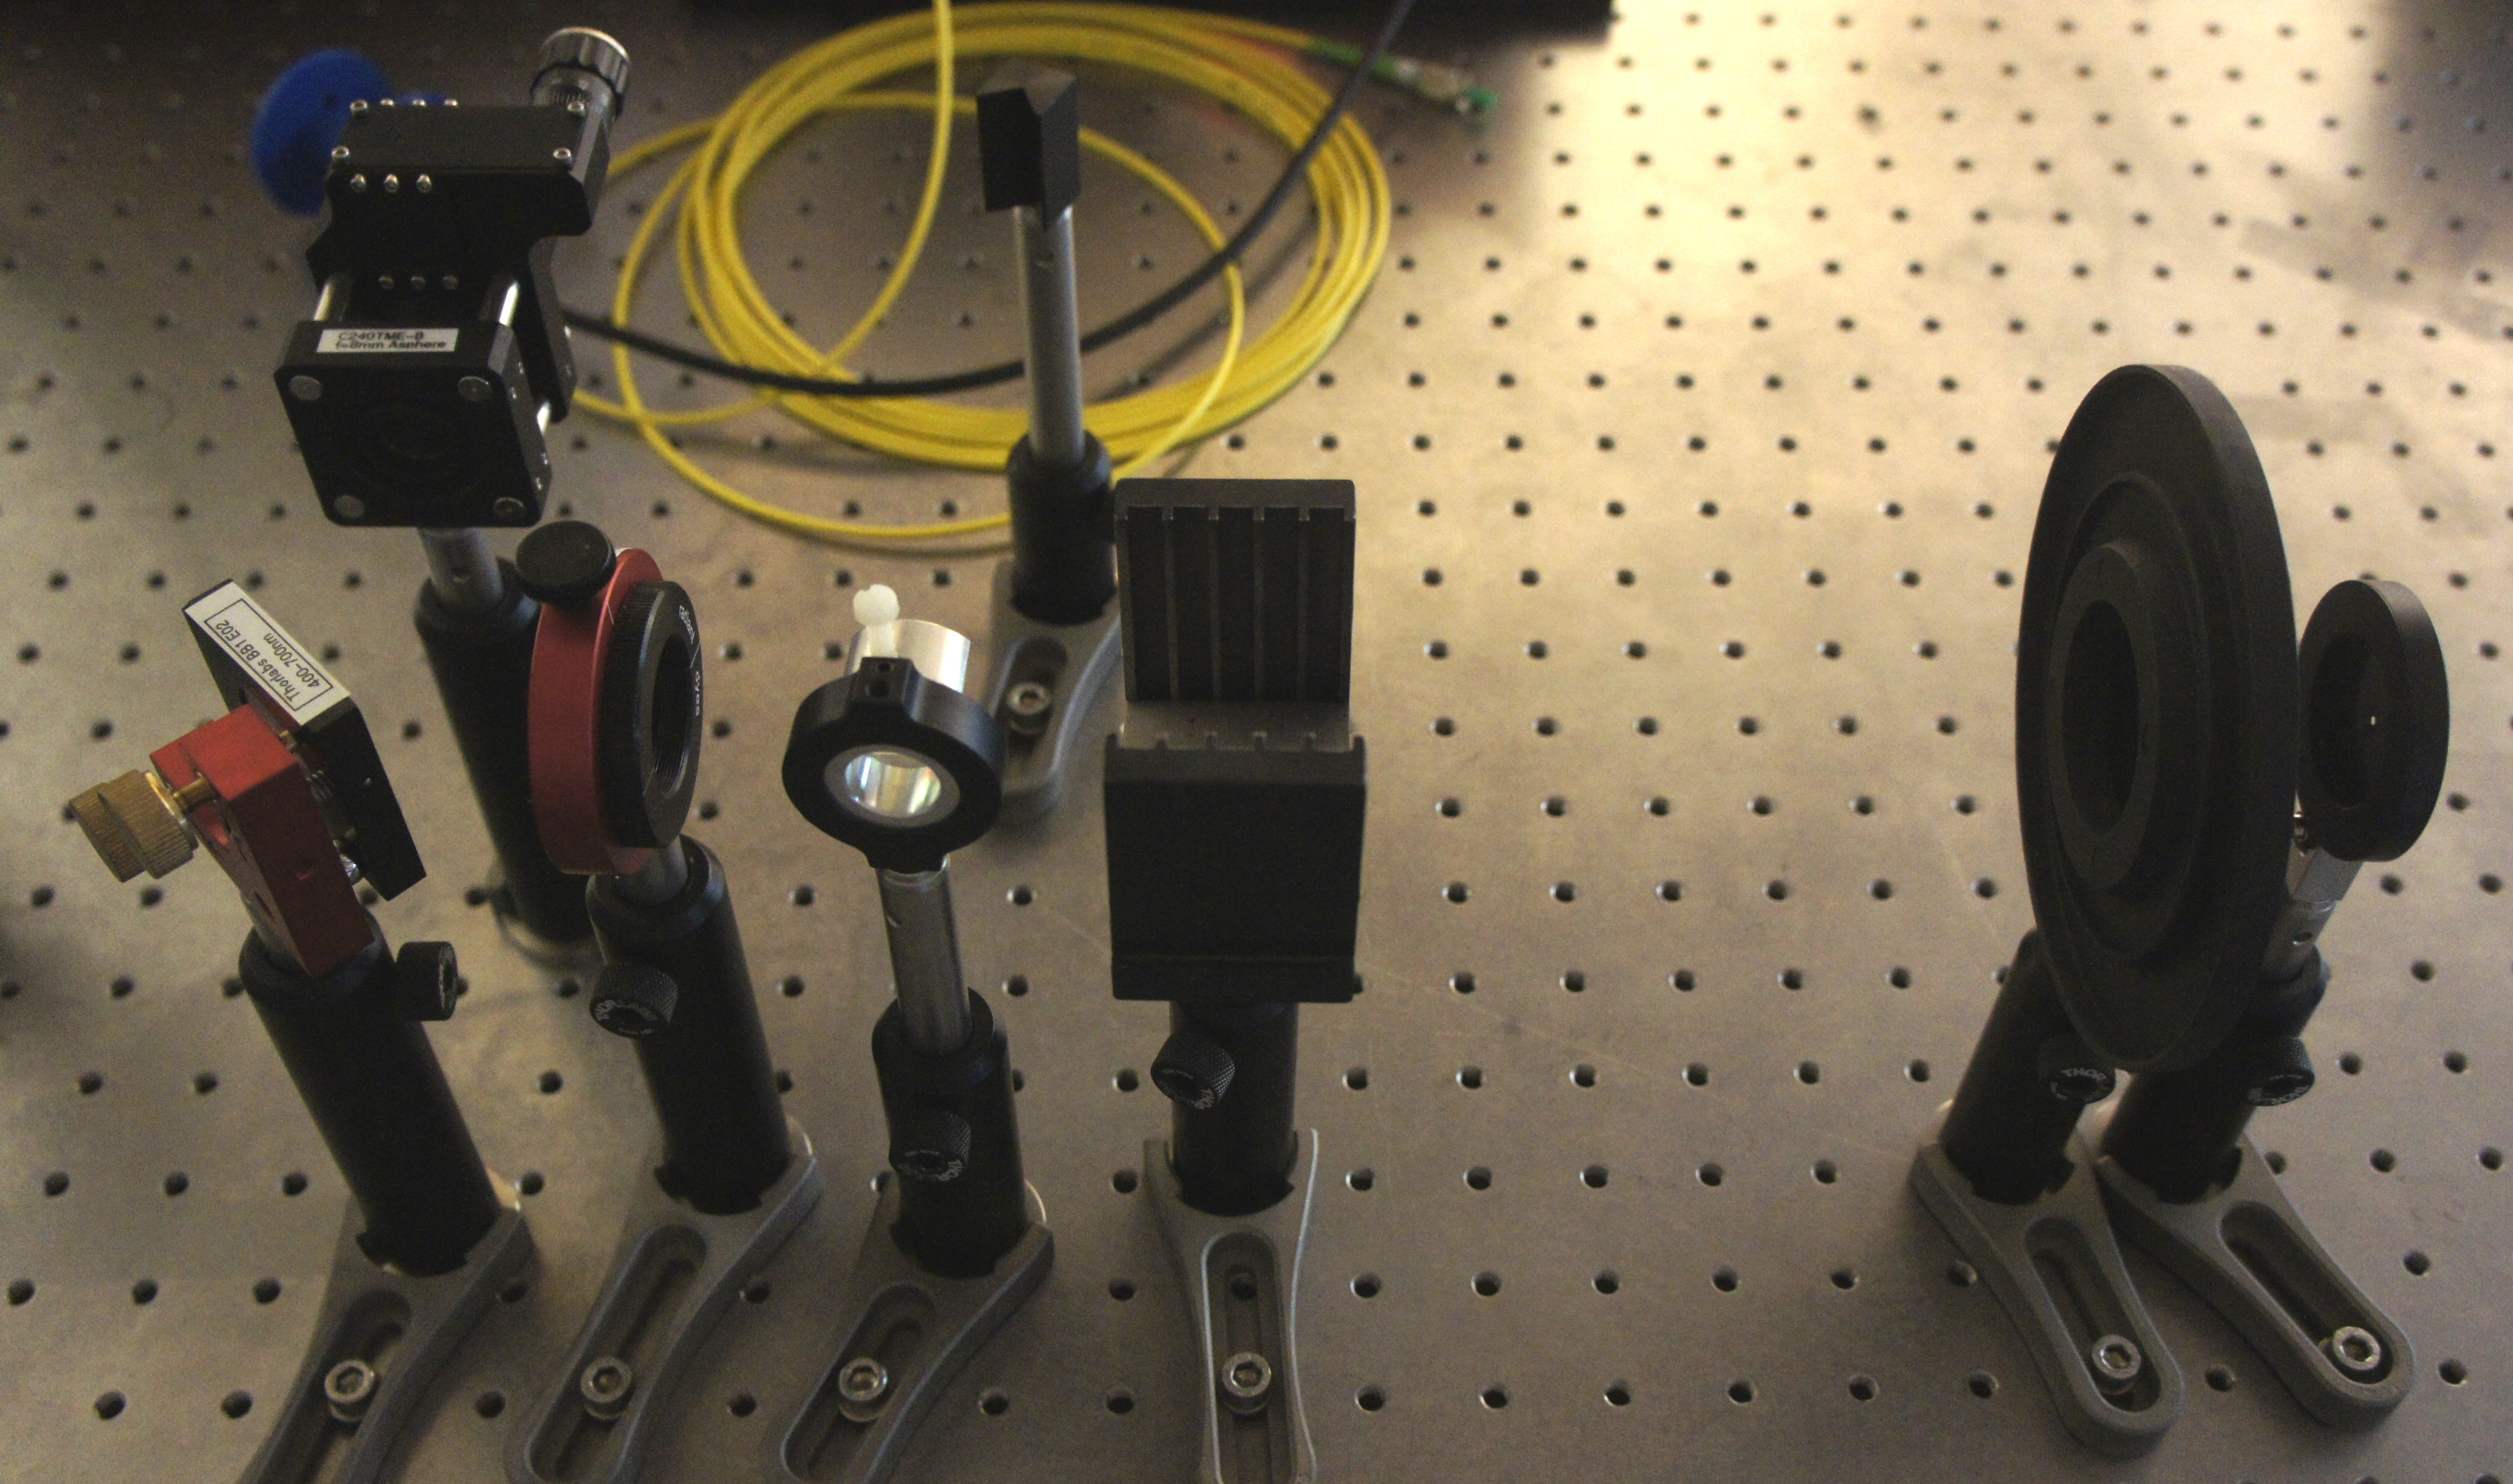
\includegraphics[width=0.7\linewidth]{images/4f-anfang.JPG}
	\caption[Vorderer Teil des 4f-Aufbaus]{
		Vorderer Teil des realisierten 4f-Aufbaus. Am rechten Bildrand ist das Pinhole hinter Linse 1 zu sehen.
	}
	\label{fig:_DSC7961}
\end{figure}

\begin{figure}[ht]
	\centering
	\includegraphicsRS[width=0.43\linewidth]{images/_DSC7988.JPG}~
	\includegraphicsRS[width=0.43\linewidth]{images/IMG_2223.jpg}
	%\vspace{2cm}\hspace{2cm}
	\caption{
		\textbf{Links:} Mode des Laserstrahls am Ende des optischen Pfades vor Einbau des Pinholes.\\
		\textbf{Rechts:} Mode des Laserstrahls am Ende des optischen Pfades nach Einbau des Pinholes.
	}
	\label{fig:_DSC7988}
\end{figure}

%TODO: Ein bisschen was über die Justierung erzählen

Als Hilfsmittel bei der Justage 




\begin{comment}
\begin{figure}
	\centering
	\includegraphicsRS[width=0.7\linewidth, angle=90]{images/_DSC7967.JPG}
	\caption{Foto des hier realisierten 4f-Aufbaus.}
	\label{fig:_DSC7967}
\end{figure}
\end{comment}

\clearpage


Nachdem der 4f-Aufbau montiert und der Verlauf des Laserstrahls im optischen Pfad optimiert war, wurden nacheinander die Objekte 1 bis 5 (siehe Abbildung~\ref{fig:Objekte-aus-Anleitungsheft}) in Form von Dias in dem Objektträger montiert.

%TODO: GgF diese Bilder je mit in die Reihe der Abbildung 9-21 Bilder machen.
\begin{figure}[h]
	\centering
	\includegraphicsRS[width=0.15\textwidth]{images/Anleitungsheft/objekt1.png}~~
	\includegraphicsRS[width=0.15\textwidth]{images/Anleitungsheft/objekt2.png}~~
	\includegraphicsRS[width=0.15\textwidth]{images/Anleitungsheft/objekt3.png}~~
	\includegraphicsRS[width=0.15\textwidth]{images/Anleitungsheft/objekt4.png}~~
	\includegraphicsRS[width=0.15\textwidth]{images/Anleitungsheft/objekt5.png}
	\caption[Die zur Messung verwendeten Diamotive]{
		Darstellung der zur Messung verwendeten Diamotive. Im Text werden diese Objekt mit Objekt 1 bis 5, von links nach rechts, bezeichnet..
	}
	\label{fig:Objekte-aus-Anleitungsheft}
\end{figure}

Anhand der Dias wurden zunächst sowohl Kamera 1, als auch Kamera 2 nachjustiert, bis ein möglichst scharfes Bild auf dem über das Programm \textit{uc480 Viewer-DCC1545M-ID} angeschlossenen Bildschirm zu erkennen war. Mit den beiden Kameras wurden nacheinander für jedes der Objekte Aufnahmen in der Abbildungsebene und zugehörig zu jeder Einstellung auch in der Fourierebene gemacht (Siehe Abbildungen~\ref{fig:example1}-\ref{fig:example16}). 


%TODO: zwischen den Bildern muss eine kleine Lücke sein. Würde vorschlagen lieber die Originale (ggF zugeschnitten) zu nehmen und über zwei \includegraphics  einzubinden. Dies gilt für alle Bilder bis Abbildung 21. Zusätzlich sollten ggF alle diese Bilder noch mal in eine Abbildung, da sie ja auch alle die gleich Caption haben.

%TODO: ....tut mir wahnsinnig leid - ich habs nicht hingekriegt. :( also das einfügen der bilder hat nich geklappt


\begin{figure}[h]
	\centering
	%\includegraphicsRS[width=0.7\linewidth]{images/example1.png}
	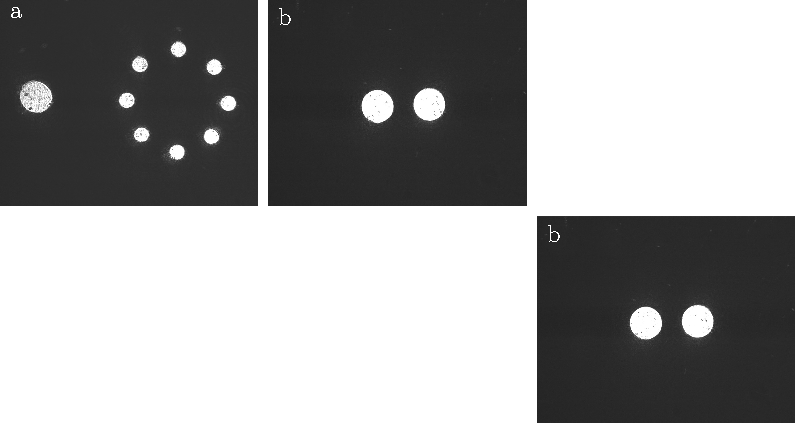
\includegraphics{images/ergebniss_ex1/abb.pdf}
	\caption{
		Beispiel von Abbildung (links) und Fourierspektrum (rechts) für Objekt 1.
	}
	\label{fig:example1}
\end{figure}

\begin{figure}[h]
	\centering
	\includegraphicsRS[width=0.7\linewidth]{images/example2.png}
	\caption{Beispiel von Abbildung (links) und Fourierspektrum (rechts) für Objekt 2}
	\label{fig:example2}
\end{figure}

\begin{figure}[h]
	\centering
	\includegraphicsRS[width=0.7\linewidth]{images/example3.png}
	\caption{Beispiel einer anderen Abbildung (links) und entsprechendes Fourierspektrum (rechts) für Objekt 2}
	\label{fig:example3}
\end{figure}

\begin{figure}[h]
	\centering
	\includegraphicsRS[width=0.7\linewidth]{images/example13.png}
	\caption{Beispiel von Abbildung (links) und Fourierspektrum (rechts) für Objekt 3}
	\label{fig:example13}
\end{figure}

\begin{figure}[h]
	\centering
	\includegraphicsRS[width=0.7\linewidth]{images/example4.png}
	\caption{Beispiel von Abbildung (links) und Fourierspektrum (rechts) für Objekt 4}
	\label{fig:example4}
\end{figure}

\begin{figure}[h]
	\centering
	\includegraphicsRS[width=0.7\linewidth]{images/example9.png}
	\caption{Beispiel einer weiteren Abbildung (links) und entsprechendes Fourierspektrum (rechts) für Objekt 4}
	\label{fig:example9}
\end{figure}

\begin{figure}[h]
	\centering
	\includegraphicsRS[width=0.7\linewidth]{images/example16.png}
	\caption{Beispiel von Abbildung (links) und Fourierspektrum (rechts) für Objekt 5}
	\label{fig:example16}
\end{figure}


\clearpage\newpage %TODO: Remove
Wie die Abbildungen \ref{fig:example1} bis \ref{fig:example16} zeigen, konnte hier beobachtet werden, dass die aus der Theorie zu erwartenden Fourierspektren mit Kamera 2 in der Fourierebene tatsächlich sichtbar gemacht werden konnten. 
Zudem wurden für die Objekte 4 und 5 verschiedene Filter in die Fourierebene gestellt und Aufnahmen der Kamera 1 in der Abbildungsebene gemacht. Für Objekt 4 wurde hierzu ein Tiefpass und mehrere Breitbandfilter verwendet. Für Objekt 5 wurde ein Halbebenenfilter horizontal, vertikal und diagonal in die Fourierebene gehalten. \\


\begin{figure}[h]
	\centering
	\includegraphicsRS[width=0.7\linewidth]{images/example10_Filter1B.png}
	\caption{
		\textbf{Links:} Beispielaufnahme von Objekt 4 aus der Abbildungsebene.\\
		\textbf{Rechts:} Aufnahme des gleichen Objekts aus der Abbildungsebene mit Filter 1B in der Fourierebene}
	\label{fig:example10_Filter1B}
\end{figure}

\begin{figure}[h]
	\centering
	\includegraphicsRS[width=0.7\linewidth]{images/example11_Filter1C.png}
	\caption{
		\textbf{Links:} Beispielaufnahme von Objekt 4 aus der Abbildungsebene.\\
		\textbf{Rechts:} Aufnahme des gleichen Objekts aus der Abbildungsebene mit Filter 1C in der Fourierebene
	}
	\label{fig:example11_Filter1C}
\end{figure}

\begin{figure}[h]
	\centering
	\includegraphicsRS[width=0.7\linewidth]{images/example12_Filter1D.png}
	\caption{links: Beispielaufnahme von Objekt 4 aus der Abbildungsebene. Rechts: Aufnahme des gleichen Objekts aus der Abbildungsebene mit Filter 1D in der Fourierebene}
	\label{fig:example12_Filter1D}
\end{figure}

\begin{figure}[h]
	\centering
	\includegraphicsRS[width=0.7\linewidth]{images/example17.png}
	\caption{links: Beispielaufnahme von Objekt 4 aus der Abbildungsebene. Rechts: Aufnahme des gleichen Objekts aus der Abbildungsebene mit vertikalem Halbebenenfilter in der Fourierebene}
	\label{fig:example17}
\end{figure}

\begin{figure}[h]
	\centering
	\includegraphicsRS[width=0.7\linewidth]{images/example18.png}
	\caption{links: Beispielaufnahme von Objekt 4 aus der Abbildungsebene. Rechts: Aufnahme des gleichen Objekts aus der Abbildungsebene mit vertikalem und diagonalem Halbebenenfilter in der Fourierebene}
	\label{fig:example18}
\end{figure}

\begin{figure}[h]
	\centering
	\includegraphicsRS[width=0.7\linewidth]{images/example19.png}
	\caption{
		\textbf{Links:} Beispielaufnahme von Objekt 4 aus der Abbildungsebene.\\
		\textbf{Rechts:} Aufnahme des gleichen Objekts aus der Abbildungsebene mit horizontalem Halbebenenfilter in der Fourierebene.
	}
	\label{fig:example19}
\end{figure}

\clearpage\newpage %TODO: Remove
Als Nächstes wurde die Abbildung eines Fingerabdrucks auf einem Glasplättchen zunächst ohne Filter aufgenommen. Hierbei war in der Abbildungsebene relativ wenig zu erkennen (siehe Abbildung \ref{fig:example20_Hochpass}, links). Anschließend wurde die Abbildung mit einem in der Fourierebene befindlichen Hochpass- und einem Halbebenenfilter aufgenommen. Zudem wird mit Kamera 2 das Fourierspektrum des Fingerabdrucks photographiert. Zu beobachten war hier, dass die Konturen des Fingerabdrucks in der Abbildung mit Hilfe der Filter deutlich besser erkennbar gemacht werden konnten (vgl Abbildung \ref{fig:example20_Hochpass}, rechts).\\


\begin{figure}[h]
	\centering
	\includegraphicsRS[width=0.6\linewidth]{images/example20_Hochpass.png}\\
	\includegraphicsRS[width=0.6\linewidth]{images/example21_Halbebenenfilter.png}
	%TODO: Nur eines dieser Bilder!
	\caption{
		\textbf{Links:} Aufnahmen des Fingerabdrucks aus der Abbildungsebene.\\
		\textbf{Rechts:} Aufnahmen des Fingerabdrucks aus der Abbildungsebene mit Hochpassfilter in der Fourierebene.
	}
	\label{fig:example20_Hochpass}
\end{figure}

Als Letztes wurde ein Teelicht auf die Position des Objektträgers gestellt und ein Halbebenenfilter in der Fourierebene installiert. Mit Kamera 1 wurden mehrere Abbildungen aufgenommen, um die Strömungsbewegungen oberhalb der Flamme beobachten zu können. Zum Vergleich wurde zudem eine Aufnahme mit Halbebenenfilter, jedoch ohne Teelicht gemacht (siehe Abb.~\ref{fig:Halbebenenfilter_mit_und_ohne_Teelicht}). Auf dieser Beispielaufnahme sind deutliche Verzerrungen des Lichts aufgrund der Luftströmungen über der Flamme des Teelichts zu erkennen. 

\begin{figure}[h]
	\centering
	\includegraphicsRS[width=0.7\linewidth]{images/example22_Halbebenenfilter_mit_und_ohne_Teelicht.png}
	\caption[Schlieren]{
		\textbf{Links:} Aufnahme aus der Abbildungsebene mit Halbebenenfilter in der Fourierebene.\\
		\textbf{Rechts:} Eine Zweite Aufnahme mit Halbebenenfilter in der Fourierebene und Teelicht an der Position des Objektträgers.}
	\label{fig:Halbebenenfilter_mit_und_ohne_Teelicht}
\end{figure}

\begin{comment}
\begin{figure}
	\centering
	\includegraphicsRS[width=0.7\linewidth]{images/example23_Halbebenenfilter_mit_und_ohne_Teelicht.png}
	\caption{
		\textbf{Links:} Aufnahme aus der Abbildungsebene mit Halbebenenfilter in der Fourierebene.
		\textbf{Rechts:} Erneute Aufnahme mit Halbebenenfilter in der Fourierebene, dieses Mal mit Teelicht an der Position des Objektträgers.
	}
	\label{fig:example23_Halbebenenfilter_mit_und_ohne_Teelicht}
\end{figure}
\end{comment}


